\chapter{Design}\label{chap:design}
\section{Overview}
This chapter provides a description of the whole JSMapper project architecture design, and the relationship between the different components that take part of it.

As seen at the end of chapter \ref{chap:preanalysis}, JSMapper main component is a kernel module implementing an special event handler for joystick-type devices. Additionally, it includes a couple more components:
\begin{itemize}
	\item A C++ library, which wraps access to the underlying kernel module through a set of useful classes.
	\item Some userspace tools, which are used to interact with the kernel module from the command line.
\end{itemize}

The following sections provide an in-depth explanation of the components above.

\section{Kernel module}
As yet mentioned, the core of JSMapper is implemented using a kernel module, named \emph{jsmapperdev}. This core is compiled against the kernel sources, then installed along with the other kernel modules so it can be automatically loaded by the system.

The module in itself is internally divided in the 3 components:
\begin{itemize}
	\item \emph{Frontend}: it handles the whole module initialization and registration into the input core. It handles also the kernel notifications such as target device connection \& disconnection, and the processing of event filtering function and API IOCTL calls.
	\item \emph{Core}: it handles the data structures needed to map device buttons and axes to mouse and keyboard actions.
	\item \emph{Event generator}: it implements the virtual event generator, which is used to inject the ``fake'' into the input core.
\end{itemize}

Figure \ref{fig:kernel_module_components} illustrates the relationship between the above components:
\begin{figure}[htb]
\centering
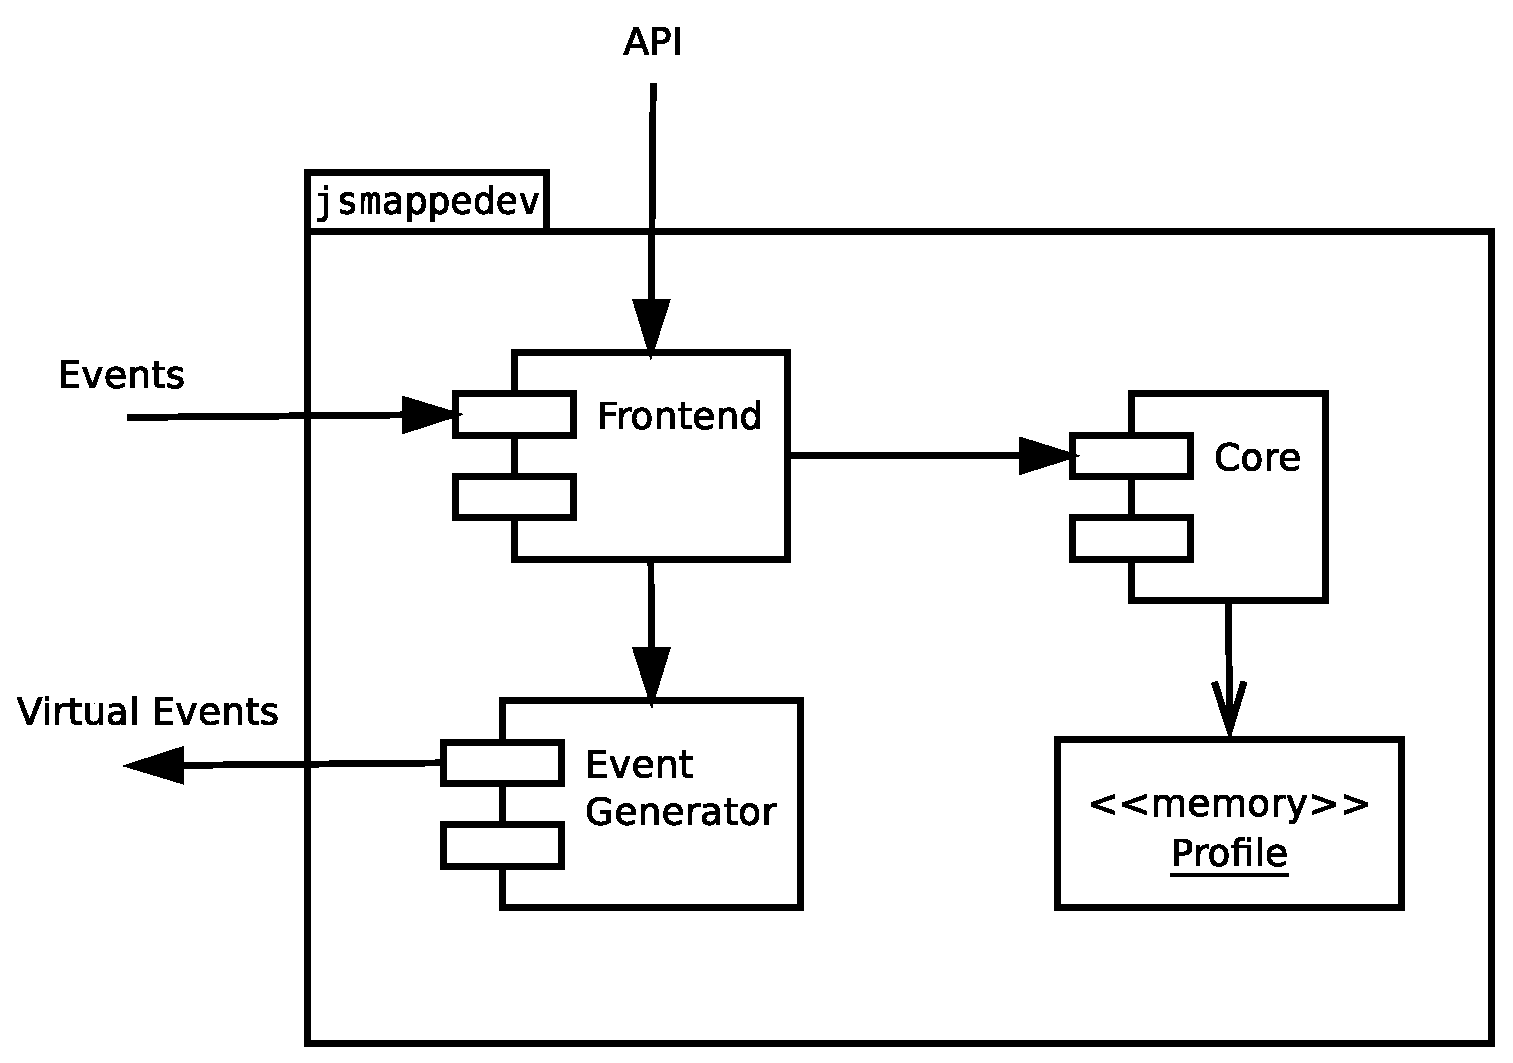
\includegraphics[width=0.7\textwidth]{kernel_module_components}
\caption{Kernel module components}
\label{fig:kernel_module_components}
\end{figure}


\subsection{Frontend}
The module frontend contains most of the \emph{glue} code needed to properly implement a Linux kernel driver. This is, it's the responsible of actually registering the module, receiving notifications on devices being plugged and/or unplugged, etc...

More specifically, the module frontent performs the following tasks:
\begin{itemize}
 \item \emph{Module initialization}: registering the module as an event handler filter for joystick type devices, in the same way \emph{joydev} module does. The virtual event generator is also created during module initialization.
 \item \emph{Device detection}: device connection and disconnection notifications are also handled by the frontend. For new devices being plugged in, it creates an associated \emph{jsmap} node for it, which will be used to \emph{program} the device using the API. For devices being removed, it simply destroys and cleanup the previously existant associated device node.
 \item \emph{Handling API calls}: the API IOCTL calls issued to the \emph{jsmap} nodes are also received by the module frontend. Its usual role here is to copy and decode the parameters received from userspace into kernel space, then forward the call to the module \emph{core}. In some cases, it will also reencode and copy back to userspace the data to return, if any.
 \item \emph{Event filtering}: events sent by the associated hardware device driver are also received by the frontend, who performs the filtering and mapping into actions (more on this below).
 \item \emph{Cleanup}: finally, cleaning up of all the associated resources at module unloading is also performed by the this component. This includes freeing all associated structures, device nodes, destroying the event generator, and finally unregistering the module from the chain of input event handlers.
\end{itemize}

\subsection{Core}
The core contains all the needed structures to keep track of the association between device elements (buttons, axes) and target actions.

On device connection, the frontend creates an initializes an instance of the ``core'' structure (a \emph{jsmapdev\_core} struct, specifically) for that device, which then gets associated to the \emph{jsmap} device node also created for the attached device. 

The ``core'' structure for a device can be then modified by means of API IOCTL calls made to the matching \emph{jsmap} device.


\subsection{Event generator}
Also during module initialization, a \emph{virtual event generator} is created: this is done by registering a new input ``device'' into input core, just as any true hardware device driver does. Only difference is that in this case the device is not attached to any ``real'' bus, but to a ``virtual'' one.

Other than that, the event generator announces itself as capable of producing keyboard and mouse events, so the system reacts to it just as it would react if a real keyboard and mouse would have been attached to the system: by creating appropiate input event handlers that will render the device visible to userspace (i.e., X11 server will start processing inputs from it without any further intervention, thanks to HAL \& D-BUS).


\subsection{Event filtering}
Event filtering is performed collaboratively between the three sub-components of the kernel module:
\begin{itemize}
 \item Module frontend receives events through the \emph{filter} callback function declared when registering the event handler.
 \item The filter function checks core to see if the source button (or axis) has any action mapped to it.
 \item If so, then it launches the simulated action through the event generator, then discards the original event thus avoiding \emph{joydev} handler processing it. 
\end{itemize}

Figure \ref{fig:kernel_event_filtering} displays the path followed by an event, since its inception on the hardware device, the filtering through \emph{jsmapperdev}, and its final destination into \emph{joydev} (the standard input handler for joystick devices), which in its turn forwards it to userspace through its own API:

\begin{figure}[htb]
\centering
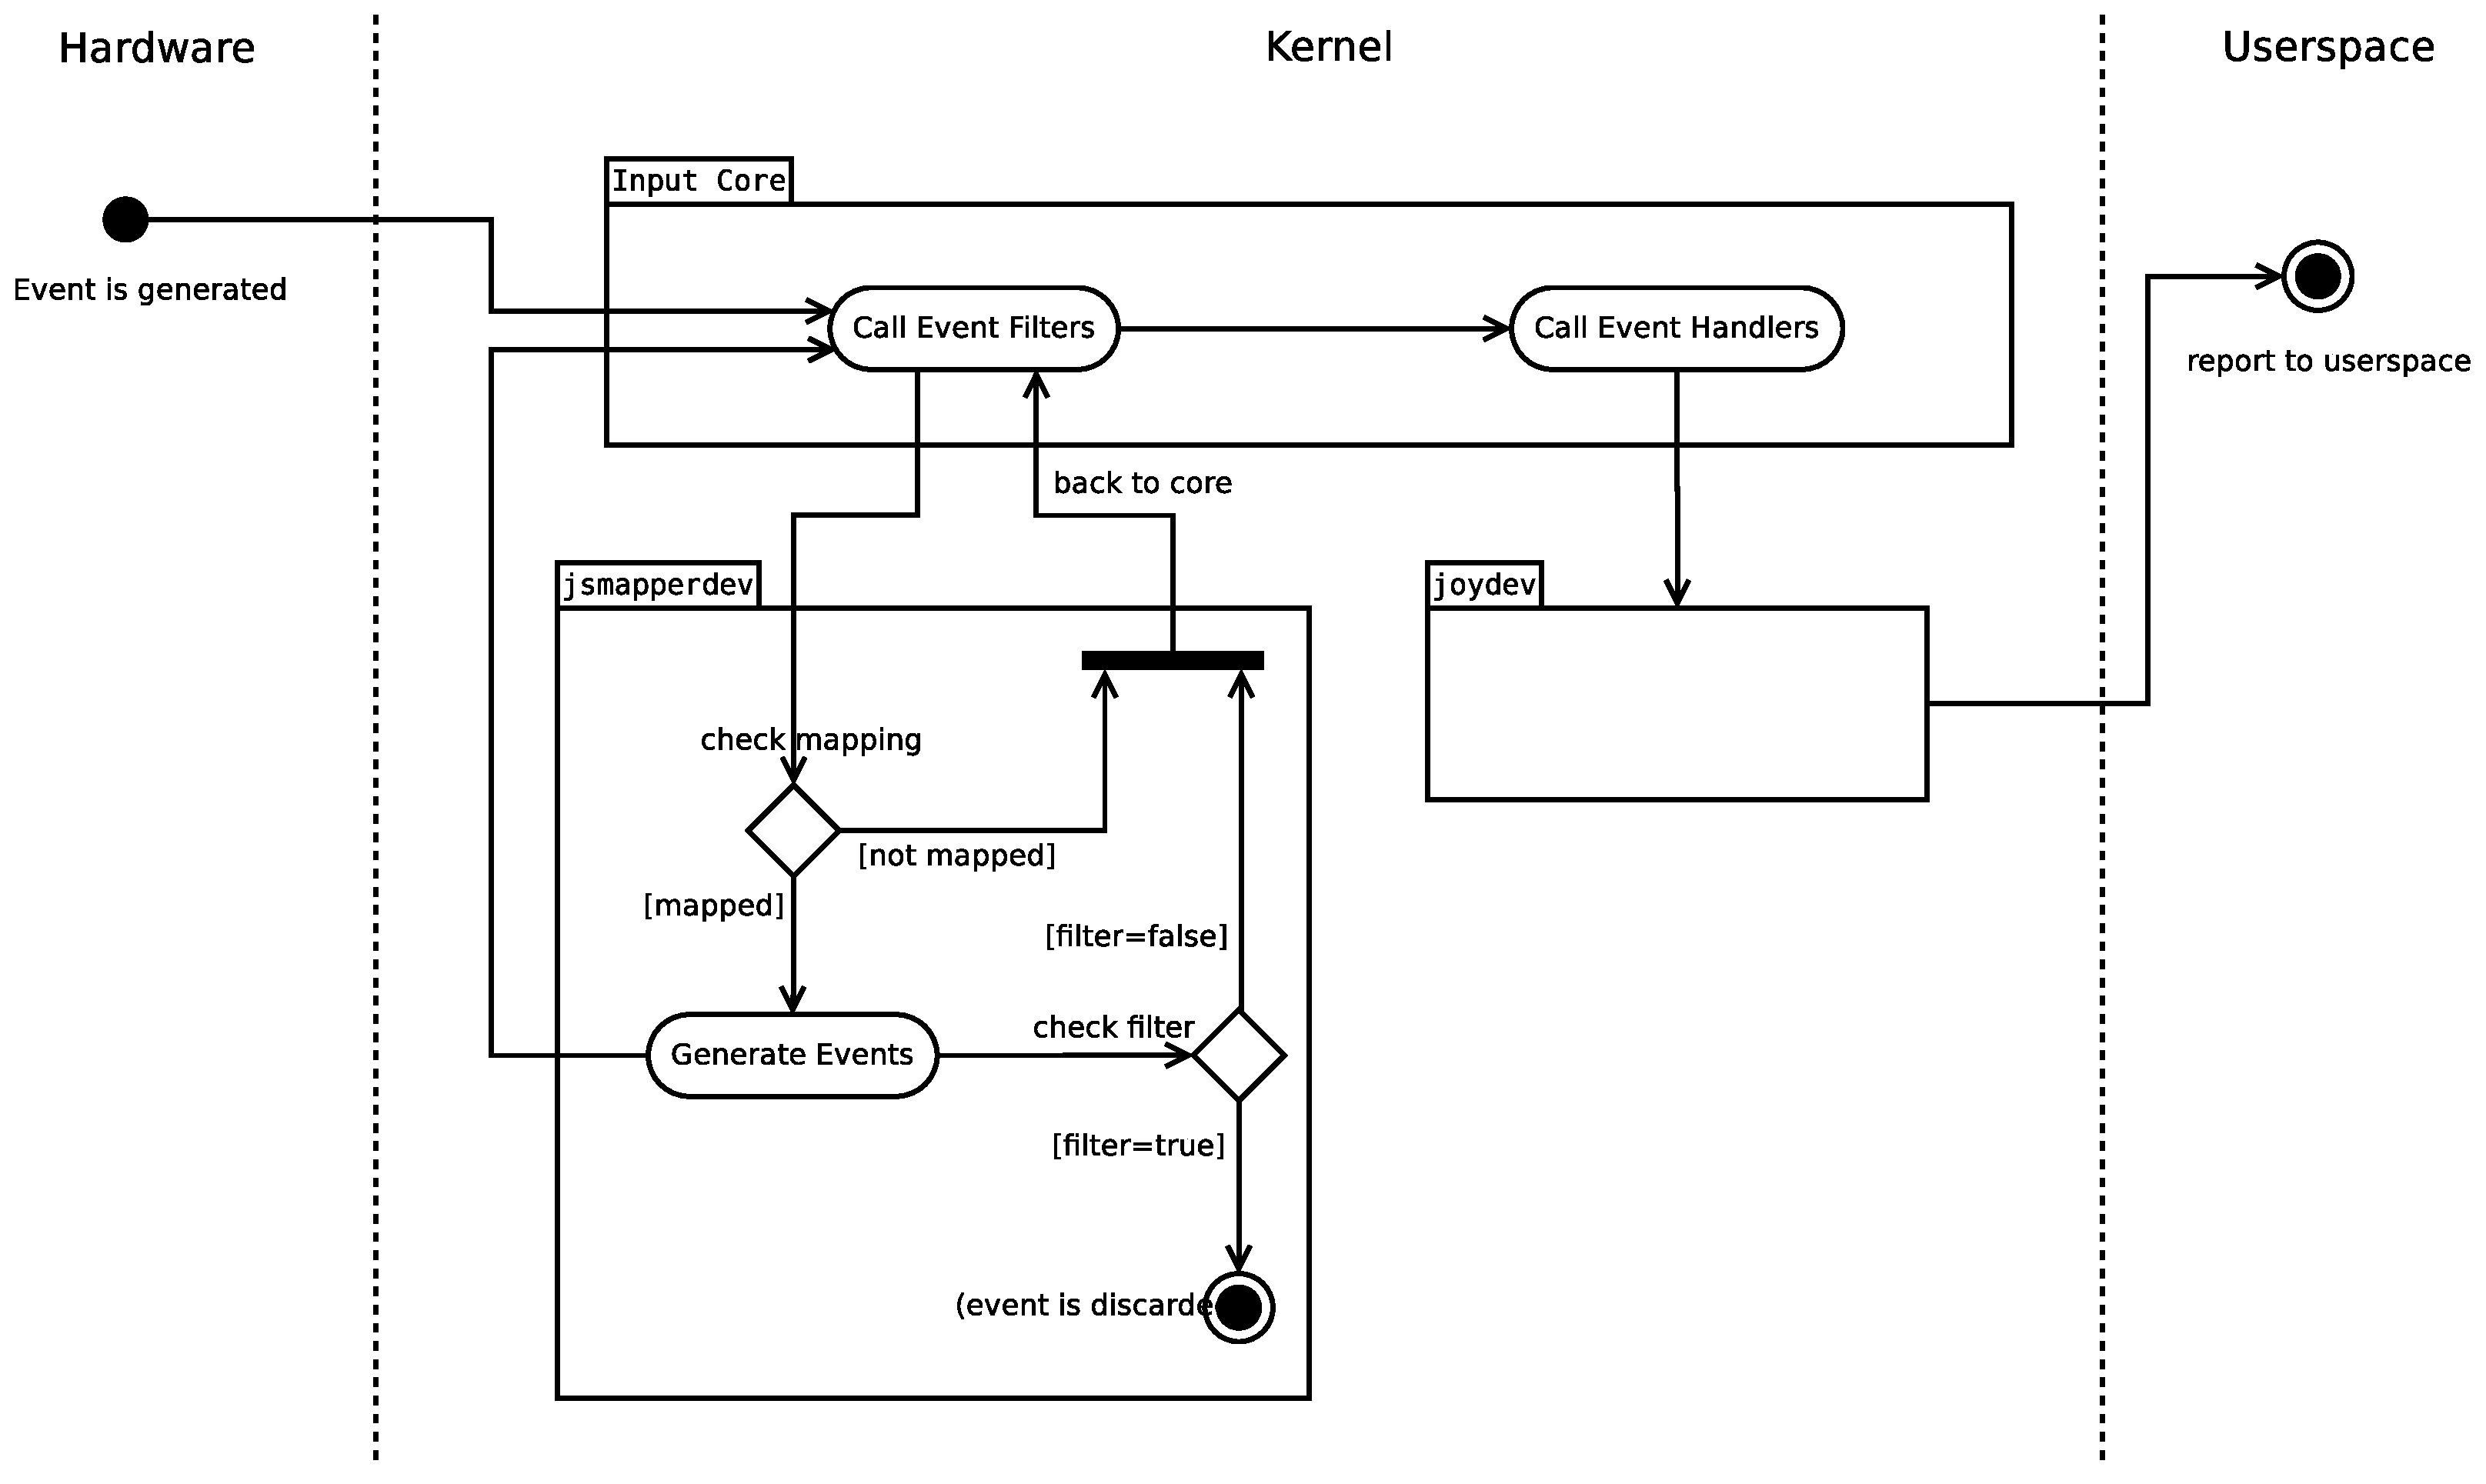
\includegraphics[width=1.0\textwidth]{kernel_event_filtering}
\caption{Event filtering flowchart}
\label{fig:kernel_event_filtering}
\end{figure}

As seen on the figure, generated events get also injected into input core in the exact same way that ``real'' events do. The \emph{jsmapperdev} module recognizes its own ``fake'' events and let them pass without any filtering, to avoid recursive calls.


\section{C/C++ library}
In order to make access to the module API easier from a developer's point of view, the project features also a C++ class library that encapsulates the access to the IOCTL API calls, using easy-to-use classes to build up profiles programatically profiles and send them to the driver.

In addition, the library provides also useful methods to save \& restore the profiles as XML files.

Here's a summary of the classes provided by the library:
\begin{itemize}
 \item \emph{Device} class: wraps access to \emph{jsmap} device nodes, providing services to query associated device status and attributes, and setting up action mapping.
 \item \emph{Action} class and subclasses: provide an easy way to create the actions to be associated to device elements.
 \item \emph{Mode} class: represents a set o assignments between device elements (buttons, axes) and actions to launch for them. A \emph{Mode} object might contain an arbitrary number of child submodes and, unless it's \emph{root} mode, an activation \emph{Condition} object.
 \item \emph{Profile} class: glues altogether by contaning the \emph{root} mode (plus their submodes, if any), and provides the XML serialization services needed to load \& save profiles from \&to disk files. 
\end{itemize}

All classes are contained into \emph{jsmapper} namespace, for name collision avoidance.

